\documentclass{extbook}[14pt]
\usepackage{multicol, enumerate, enumitem, hyperref, color, soul, setspace, parskip, fancyhdr, amssymb, amsthm, amsmath, latexsym, units, mathtools}
\everymath{\displaystyle}
\usepackage[headsep=0.5cm,headheight=0cm, left=1 in,right= 1 in,top= 1 in,bottom= 1 in]{geometry}
\usepackage{dashrule}  % Package to use the command below to create lines between items
\newcommand{\litem}[1]{\item #1

\rule{\textwidth}{0.4pt}}
\pagestyle{fancy}
\lhead{}
\chead{Answer Key for Makeup Progress Quiz 2 Version A}
\rhead{}
\lfoot{5763-3522}
\cfoot{}
\rfoot{Spring 2021}
\begin{document}
\textbf{This key should allow you to understand why you choose the option you did (beyond just getting a question right or wrong). \href{https://xronos.clas.ufl.edu/mac1105spring2020/courseDescriptionAndMisc/Exams/LearningFromResults}{More instructions on how to use this key can be found here}.}

\textbf{If you have a suggestion to make the keys better, \href{https://forms.gle/CZkbZmPbC9XALEE88}{please fill out the short survey here}.}

\textit{Note: This key is auto-generated and may contain issues and/or errors. The keys are reviewed after each exam to ensure grading is done accurately. If there are issues (like duplicate options), they are noted in the offline gradebook. The keys are a work-in-progress to give students as many resources to improve as possible.}

\rule{\textwidth}{0.4pt}

\begin{enumerate}\litem{
Solve the rational equation below. Then, choose the interval(s) that the solution(s) belongs to.
\[ \frac{-3}{-4x -6} + 6 = \frac{-9}{12x + 18} \]The solution is \( x = -1.750 \), which is option D.\begin{enumerate}[label=\Alph*.]
\item \( x_1 \in [-2.75, -0.75] \text{ and } x_2 \in [-2.25,-0.25] \)

$x = -1.750 \text{ and } x = -1.250$, which corresponds to getting the correct solution and believing there should be a second solution to the equation.
\item \( \text{All solutions lead to invalid or complex values in the equation.} \)

This corresponds to thinking $x = -1.750$ leads to dividing by zero in the original equation, which it does not.
\item \( x \in [0.25,3.25] \)

$x = 1.250$, which corresponds to not distributing the factor $-4x -6$ correctly when trying to eliminate the fraction.
\item \( x \in [-1.75,0.25] \)

* $x = -1.750$, which is the correct option.
\item \( x_1 \in [-2.75, -0.75] \text{ and } x_2 \in [0.25,2.25] \)

$x = -1.750 \text{ and } x = 1.250$, which corresponds to getting the correct solution and believing there should be a second solution to the equation.
\end{enumerate}

\textbf{General Comment:} Distractors are different based on the number of solutions. Remember that after solving, we need to make sure our solution does not make the original equation divide by zero!
}
\litem{
Determine the domain of the function below.
\[ f(x) = \frac{4}{20x^{2} -35 x + 15} \]The solution is \( \text{All Real numbers except } x = 0.750 \text{ and } x = 1.000. \), which is option C.\begin{enumerate}[label=\Alph*.]
\item \( \text{All Real numbers except } x = a, \text{ where } a \in [11.91, 12.78] \)

All Real numbers except $x = 12.000$, which corresponds to removing a distractor value from the denominator.
\item \( \text{All Real numbers.} \)

This corresponds to thinking the denominator has complex roots or that rational functions have a domain of all Real numbers.
\item \( \text{All Real numbers except } x = a \text{ and } x = b, \text{ where } a \in [0.31, 0.96] \text{ and } b \in [0.94, 1.52] \)

All Real numbers except $x = 0.750$ and $x = 1.000$, which is the correct option.
\item \( \text{All Real numbers except } x = a, \text{ where } a \in [0.31, 0.96] \)

All Real numbers except $x = 0.750$, which corresponds to removing only 1 value from the denominator.
\item \( \text{All Real numbers except } x = a \text{ and } x = b, \text{ where } a \in [11.91, 12.78] \text{ and } b \in [24.72, 25.13] \)

All Real numbers except $x = 12.000$ and $x = 25.000$, which corresponds to not factoring the denominator correctly.
\end{enumerate}

\textbf{General Comment:} Recall that dividing by zero is not a real number. Therefore the domain is all real numbers \textbf{except} those that make the denominator 0.
}
\litem{
Choose the equation of the function graphed below.

\begin{center}
    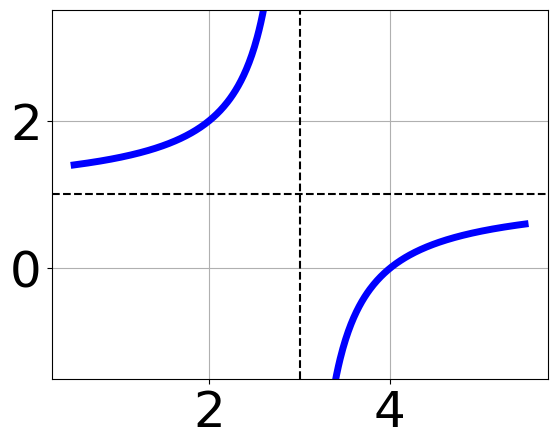
\includegraphics[width=0.5\textwidth]{../Figures/rationalGraphToEquationCopyA.png}
\end{center}


The solution is \( f(x) = \frac{-1}{x - 3} + 1 \), which is option B.\begin{enumerate}[label=\Alph*.]
\item \( f(x) = \frac{1}{(x + 3)^2} + 1 \)

Corresponds to thinking the graph was a shifted version of $\frac{1}{x^2}$, using the general form $f(x) = \frac{a}{x+h}+k$, and the opposite leading coefficient.
\item \( f(x) = \frac{-1}{x - 3} + 1 \)

This is the correct option.
\item \( f(x) = \frac{-1}{(x - 3)^2} + 1 \)

Corresponds to thinking the graph was a shifted version of $\frac{1}{x^2}$.
\item \( f(x) = \frac{1}{x + 3} + 1 \)

Corresponds to using the general form $f(x) = \frac{a}{x+h}+k$ and the opposite leading coefficient.
\item \( \text{None of the above} \)

This corresponds to believing the vertex of the graph was not correct.
\end{enumerate}

\textbf{General Comment:} Remember that the general form of a basic rational equation is $ f(x) = \frac{a}{(x-h)^n} + k$, where $a$ is the leading coefficient (and in this case, we assume is either $1$ or $-1$), $n$ is the degree (in this case, either $1$ or $2$), and $(h, k)$ is the intersection of the asymptotes.
}
\litem{
Choose the equation of the function graphed below.

\begin{center}
    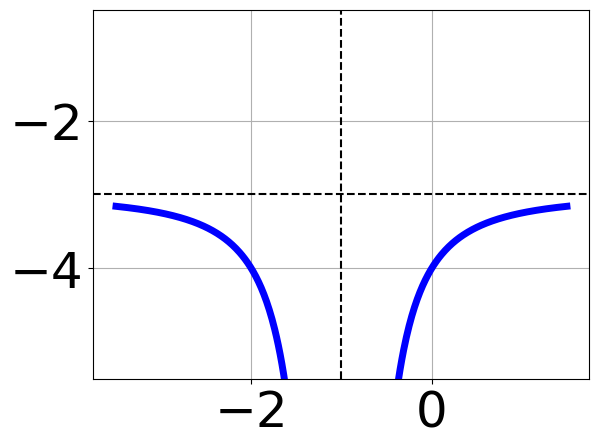
\includegraphics[width=0.5\textwidth]{../Figures/rationalGraphToEquationA.png}
\end{center}


The solution is \( f(x) = \frac{-1}{(x + 1)^2} - 3 \), which is option B.\begin{enumerate}[label=\Alph*.]
\item \( f(x) = \frac{1}{(x - 1)^2} - 3 \)

Corresponds to using the general form $f(x) = \frac{a}{(x+h)^2}+k$ and the opposite leading coefficient.
\item \( f(x) = \frac{-1}{(x + 1)^2} - 3 \)

This is the correct option.
\item \( f(x) = \frac{1}{x - 1} - 3 \)

Corresponds to thinking the graph was a shifted version of $\frac{1}{x}$, using the general form $f(x) = \frac{a}{(x+h)^2}+k$, and the opposite leading coefficient.
\item \( f(x) = \frac{-1}{x + 1} - 3 \)

Corresponds to thinking the graph was a shifted version of $\frac{1}{x}$.
\item \( \text{None of the above} \)

This corresponds to believing the vertex of the graph was not correct.
\end{enumerate}

\textbf{General Comment:} Remember that the general form of a basic rational equation is $ f(x) = \frac{a}{(x-h)^n} + k$, where $a$ is the leading coefficient (and in this case, we assume is either $1$ or $-1$), $n$ is the degree (in this case, either $1$ or $2$), and $(h, k)$ is the intersection of the asymptotes.
}
\litem{
Solve the rational equation below. Then, choose the interval(s) that the solution(s) belongs to.
\[ \frac{7x}{-6x + 6} + \frac{-3x^{2}}{36x^{2} -78 x + 42} = \frac{5}{-6x + 7} \]The solution is \( \text{There are two solutions: } x = 0.556 \text{ and } x = 1.200 \), which is option C.\begin{enumerate}[label=\Alph*.]
\item \( x_1 \in [0.55, 0.62] \text{ and } x_2 \in [0.69,1.07] \)


\item \( x \in [1.16,1.18] \)


\item \( x_1 \in [0.55, 0.62] \text{ and } x_2 \in [1.07,1.48] \)

* $x = 0.556 \text{ and } x = 1.200$, which is the correct option.
\item \( x \in [1.17,1.34] \)


\item \( \text{All solutions lead to invalid or complex values in the equation.} \)


\end{enumerate}

\textbf{General Comment:} Distractors are different based on the number of solutions. Remember that after solving, we need to make sure our solution does not make the original equation divide by zero!
}
\litem{
Solve the rational equation below. Then, choose the interval(s) that the solution(s) belongs to.
\[ \frac{-9}{-6x -2} + 6 = \frac{-2}{-54x -18} \]The solution is \( x = -0.577 \), which is option B.\begin{enumerate}[label=\Alph*.]
\item \( x_1 \in [-1.4, -0.1] \text{ and } x_2 \in [-0.9,-0.3] \)

$x = -0.577 \text{ and } x = -0.528$, which corresponds to getting the correct solution and believing there should be a second solution to the equation.
\item \( x \in [-1.58,1.42] \)

* $x = -0.577$, which is the correct option.
\item \( x \in [-0.2,1.3] \)

$x = 0.090$, which corresponds to not distributing the factor $-6x -2$ correctly when trying to eliminate the fraction.
\item \( x_1 \in [-1.4, -0.1] \text{ and } x_2 \in [-0.5,0.9] \)

$x = -0.577 \text{ and } x = 0.090$, which corresponds to getting the correct solution and believing there should be a second solution to the equation.
\item \( \text{All solutions lead to invalid or complex values in the equation.} \)

This corresponds to thinking $x = -0.577$ leads to dividing by zero in the original equation, which it does not.
\end{enumerate}

\textbf{General Comment:} Distractors are different based on the number of solutions. Remember that after solving, we need to make sure our solution does not make the original equation divide by zero!
}
\litem{
Determine the domain of the function below.
\[ f(x) = \frac{4}{25x^{2} +45 x + 20} \]The solution is \( \text{All Real numbers except } x = -1.000 \text{ and } x = -0.800. \), which is option C.\begin{enumerate}[label=\Alph*.]
\item \( \text{All Real numbers except } x = a \text{ and } x = b, \text{ where } a \in [-25.34, -24.97] \text{ and } b \in [-20.13, -19.86] \)

All Real numbers except $x = -25.000$ and $x = -20.000$, which corresponds to not factoring the denominator correctly.
\item \( \text{All Real numbers except } x = a, \text{ where } a \in [-25.34, -24.97] \)

All Real numbers except $x = -25.000$, which corresponds to removing a distractor value from the denominator.
\item \( \text{All Real numbers except } x = a \text{ and } x = b, \text{ where } a \in [-1.15, -0.85] \text{ and } b \in [-0.87, -0.58] \)

All Real numbers except $x = -1.000$ and $x = -0.800$, which is the correct option.
\item \( \text{All Real numbers except } x = a, \text{ where } a \in [-1.15, -0.85] \)

All Real numbers except $x = -1.000$, which corresponds to removing only 1 value from the denominator.
\item \( \text{All Real numbers.} \)

This corresponds to thinking the denominator has complex roots or that rational functions have a domain of all Real numbers.
\end{enumerate}

\textbf{General Comment:} Recall that dividing by zero is not a real number. Therefore the domain is all real numbers \textbf{except} those that make the denominator 0.
}
\litem{
Choose the graph of the equation below.
\[ f(x) = \frac{1}{x - 3} + 1 \]The solution is the graph below, which is option A.
\begin{center}
    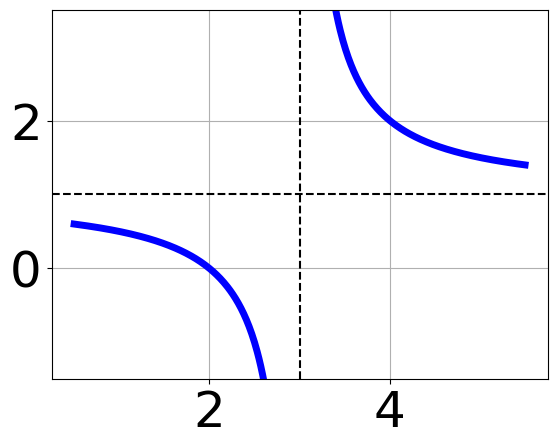
\includegraphics[width=0.3\textwidth]{../Figures/rationalEquationToGraphCopyAA.png}
\end{center}\begin{enumerate}[label=\Alph*.]
\begin{multicols}{2}
\item 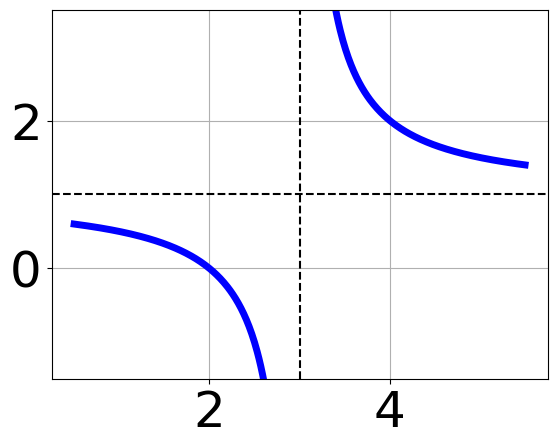
\includegraphics[width = 0.3\textwidth]{../Figures/rationalEquationToGraphCopyAA.png}
\item 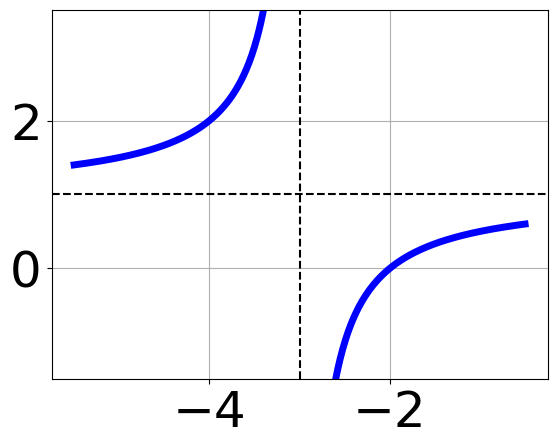
\includegraphics[width = 0.3\textwidth]{../Figures/rationalEquationToGraphCopyBA.png}
\item 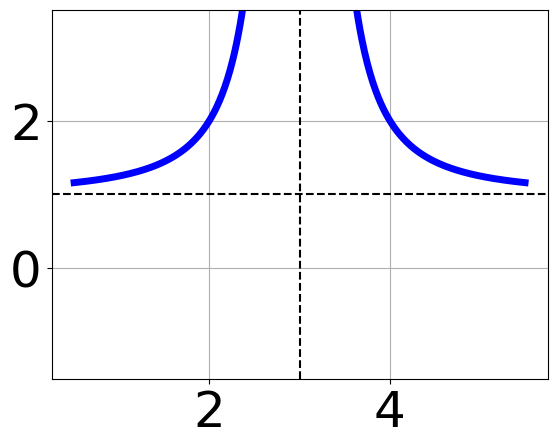
\includegraphics[width = 0.3\textwidth]{../Figures/rationalEquationToGraphCopyCA.png}
\item 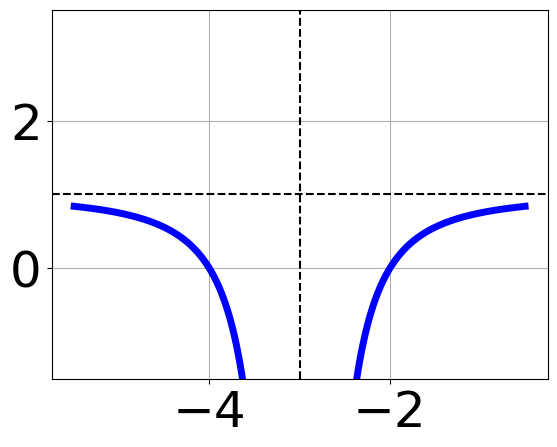
\includegraphics[width = 0.3\textwidth]{../Figures/rationalEquationToGraphCopyDA.png}
\end{multicols}\item None of the above.\end{enumerate}
\textbf{General Comment:} Remember that the general form of a basic rational equation is $ f(x) = \frac{a}{(x-h)^n} + k$, where $a$ is the leading coefficient (and in this case, we assume is either $1$ or $-1$), $n$ is the degree (in this case, either $1$ or $2$), and $(h, k)$ is the intersection of the asymptotes.
}
\litem{
Choose the graph of the equation below.
\[ f(x) = \frac{-1}{x + 3} - 3 \]The solution is the graph below, which is option B.
\begin{center}
    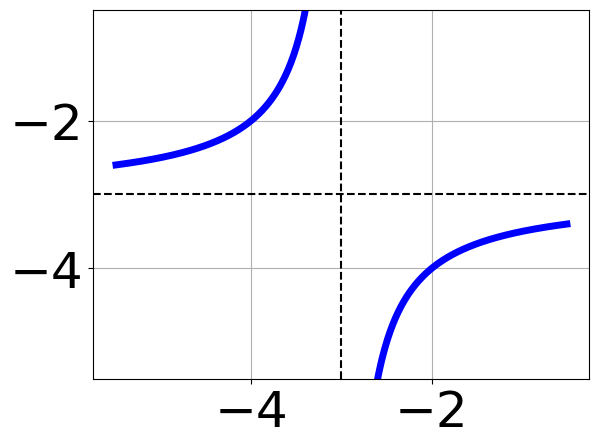
\includegraphics[width=0.3\textwidth]{../Figures/rationalEquationToGraphBA.png}
\end{center}\begin{enumerate}[label=\Alph*.]
\begin{multicols}{2}
\item 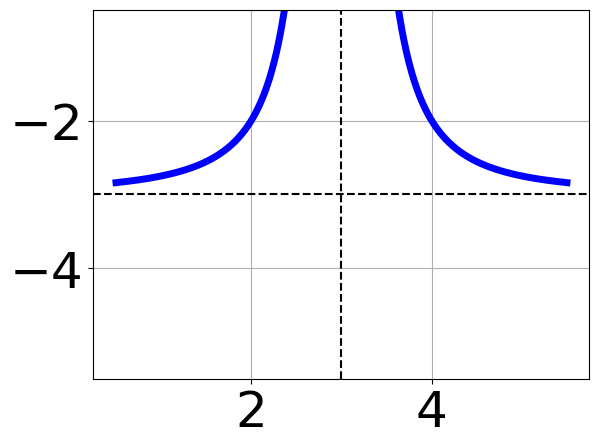
\includegraphics[width = 0.3\textwidth]{../Figures/rationalEquationToGraphAA.png}
\item 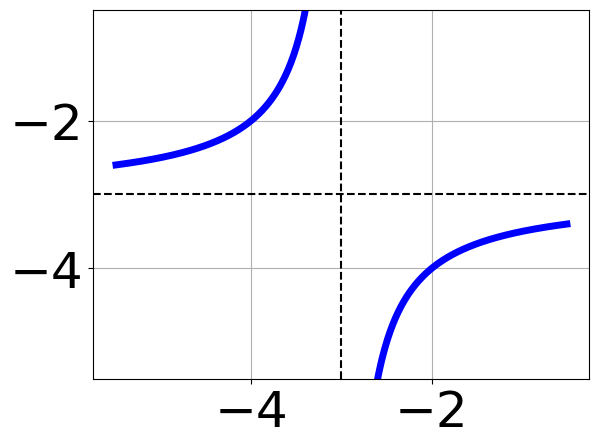
\includegraphics[width = 0.3\textwidth]{../Figures/rationalEquationToGraphBA.png}
\item 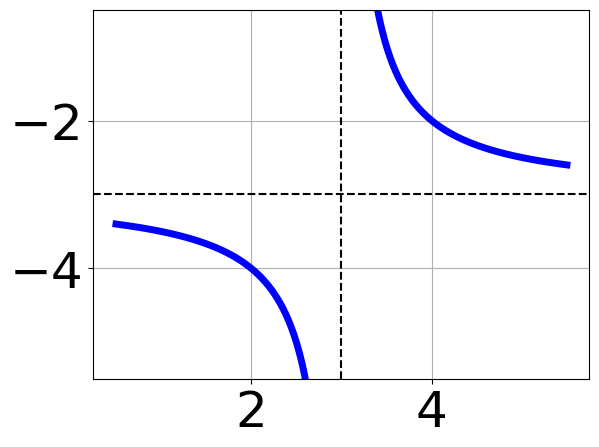
\includegraphics[width = 0.3\textwidth]{../Figures/rationalEquationToGraphCA.png}
\item 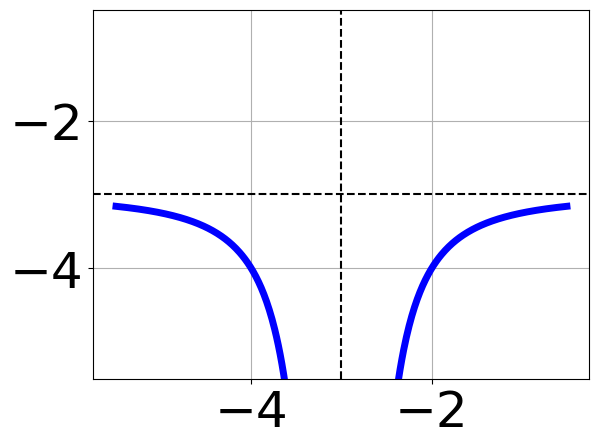
\includegraphics[width = 0.3\textwidth]{../Figures/rationalEquationToGraphDA.png}
\end{multicols}\item None of the above.\end{enumerate}
\textbf{General Comment:} Remember that the general form of a basic rational equation is $ f(x) = \frac{a}{(x-h)^n} + k$, where $a$ is the leading coefficient (and in this case, we assume is either $1$ or $-1$), $n$ is the degree (in this case, either $1$ or $2$), and $(h, k)$ is the intersection of the asymptotes.
}
\litem{
Solve the rational equation below. Then, choose the interval(s) that the solution(s) belongs to.
\[ \frac{-3x}{-5x + 2} + \frac{-3x^{2}}{30x^{2} -27 x + 6} = \frac{-3}{-6x + 3} \]The solution is \( \text{There are two solutions: } x = 0.310 \text{ and } x = 1.290 \), which is option B.\begin{enumerate}[label=\Alph*.]
\item \( x \in [1.22,1.51] \)


\item \( x_1 \in [0.25, 0.37] \text{ and } x_2 \in [1.15,2.13] \)

* $x = 0.310 \text{ and } x = 1.290$, which is the correct option.
\item \( x_1 \in [0.25, 0.37] \text{ and } x_2 \in [-1.09,0.72] \)


\item \( \text{All solutions lead to invalid or complex values in the equation.} \)


\item \( x \in [0.37,0.71] \)


\end{enumerate}

\textbf{General Comment:} Distractors are different based on the number of solutions. Remember that after solving, we need to make sure our solution does not make the original equation divide by zero!
}
\end{enumerate}

\end{document}